
\chapter{Evaluation}

In this chapter we provide detailed description of the evaluation process that we carried out for testing multiple versions of our paraphrasing approach. Considering the modular design of our paraphraser it was possible to design several experiments by adding and removing specific functionality. In scope of this project we were mainly interested in evaluating usefulness of paraphrasing options provided by our tool in context of a translation task. It was not feasible to set up user studies at early stage of the project, because there were too many versions to test. Considering that we designed an automatic evaluation system that helped us to find the most promising versions and also highlighted various issues and interesting features about our tool. We will begin this chapter by describing this automatic evaluation process. At the final stage of project we also carried out a small user study. We will show how results of this study supported our previous findings. Describing each evaluation stage we will also provide analysis and interpretation of the results.

\section{Automatic evaluation}

The design of our automatic evaluation is similar to the multiple translations technique that was described in the background chapter. Our main goal was to test whether our paraphraser can find a suitable paraphrase to a given part of machine translation output. To achieve this goal we created a large repository of test cases. Each test case contains a sentence corrupted by machine translation and a set of suggested paraphrases for different parts of this sentence. In our evaluation process we treat these suggested paraphrases as the gold standard. In order to collect this kind of test data, we artificially corrupted 1000 English (natural language) sentences from news domain (\emph{newstest2012b} dataset) by translating them into Russian and then back into English. This way the resulting English sentences were expressing the same idea as original ones. However, most of them were stylistically or grammatically incorrect. We detected different parts in original and corrupted version and passed the corrupted parts to our paraphraser. We considered the test case successful if corresponding original part was in top $n$ paraphrasing suggestions. In our experiments we considered $n = 5$, as this is the desired number of options displayed to the user. We begin this section by providing a short overview of the test case generation process, then we will provide the evaluation results. We will conclude current section by discussing problems of this evaluation type.


\subsection{Generating test cases}

In order to generate the test cases, we used the Moses toolkit to translate 1000 English (natural language) sentences into Russian. First, we generated a translation model for English - Russian pair using following command:

\begin{verbatim}
/moses-git2/scripts/training/filter-model-given-input.pl 
~/secondfilter ~/m2config.ini ~/eng.orig.result.in 
-Binarizer "/moses-git2/bin/processPhraseTable"
\end{verbatim} 

Then we used the generated model output (\texttt{~/secondfilter}) to translate sentences executing following command:

\begin{verbatim}
/moses-git2/bin/moses.2013-01-26 -mbr -mp -search-algorithm 1 
-cube-pruning-pop-limit 5000 -s 5000 -threads 24  -ttable-limit 100
-max-trans-opt-per-coverage 100 -f ~/finalfilter/moses.ini 
< /fs/vali1/wmt13-en-ru/evaluation/newstest2013.input.lc.1 > ~/rus_out_1
\end{verbatim} 

Figure 4.1 illustrates sample original English sentence (a) and it's Russian translation (b). We used a simple Python script to remove coverage information from the results in order to use it as input for Russian - English translation, sample result is illustrated on Figure 4.1 (c). Following command was used to build Russian to English translation model:

\begin{verbatim}
/moses-git2/scripts/training/filter-model-given-input.pl 
~/secondfilter ~/m2config.ini ~/rus.result.in 
-Binarizer "/moses-git2/bin/processPhraseTable"
\end{verbatim} 

Finally, we translated Russian sentences back to English by running Moses with following configurations:

\begin{verbatim}
/moses-git2/bin/moses.2013-01-26 -mbr -mp -search-algorithm 
1 -cube-pruning-pop-limit 5000 -s 5000 -threads 24  -ttable-limit 100
-max-trans-opt-per-coverage 100 -f ~/secondfilter/moses.ini 
< ~/rus.result.in > ~/en_out_new2
\end{verbatim} 

The resulting English sentence is illustrated on Figure 4.1 (d). As we can see it is different from original English input. In this case the difference is in phrases ``us states'' and ``american states''. Obviously, original phrase ``american states'' is a better translation and if our paraphraser can suggest it in top 5 results we can consider that as a successful test case. 

Considering this, we extracted all differences between original English and corrupted English sentences and stored them in our test case repository. To detect corrupted parts, we used coverage information to align parts of corrupted and original English sentences. After alignment we saved pointers to different parts. For our example, ``us states'' has coverage \texttt{|5-6|}, what corresponds to 6th and 7th words in Russian translation. As we can see from Figure 4.1 (b) these words have following coverages: \texttt{|5-5|} and \texttt{|6-6|}. These coverage information points to ``american states''. Comparing this to ``us states'' we spot the difference. We applied the same procedure for all phrases in final English translation. For each sentence we merged sequential difference intervals.

As a result we collected 2139 test cases, that were used for evaluation. While we applied this technique to collect evaluation data, it can also be seen as an alternative paraphrasing approach. Indeed, most of resulting samples were paraphrase pairs. However, this paraphrasing is very expensive and time-consuming to be used within an interactive environment. 

\begin{figure}
 \centering 
 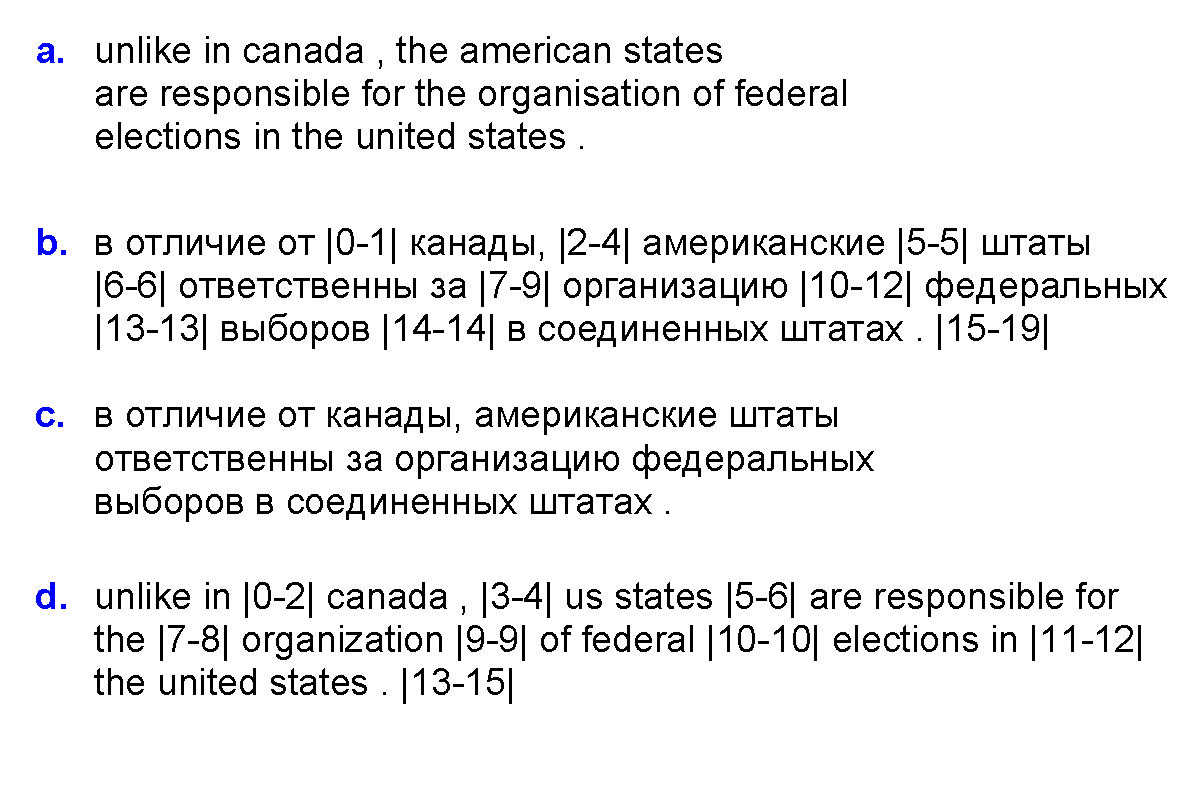
\includegraphics[scale=0.75]{g/rus-sample1.pdf}
 \caption{Resulting Russian translation}
\end{figure}

\subsection{Results of automatic evaluation}

We tested ten different versions of our approach using the test case repository we discussed in previous section. These versions differ in filters, sorters and score functions. Figure 4.2 illustrates outcome of our automatic evaluation. The first columns identify types of functions we used. Description of these functions could be found in Section 3.4. The final column contains the score, which expresses the number of successfully solved test cases out of 2139 total tests.

\subsection{Analysing automatic evaluation results}

As we can see from results illustrated on Figure 4.2, we achieve the best performance with Approach 10. This approach uses all partial filters, all score functions and all sorters in same order as listed in the table. In contrast, Approach 1 has the worst performance. For this approach we did not use any filters or sorters. However we used punctuation partial filter and score difference based score function. We consider Approach 1 as the \emph{baseline} baseline approach, because it uses only minimum required functions. Furthermore, we can see that we achieve better performance by adding language model based features. Also from the results we can see that using sorters significantly improves the performance of paraphraser.


\begin{figure}
 \centering 
 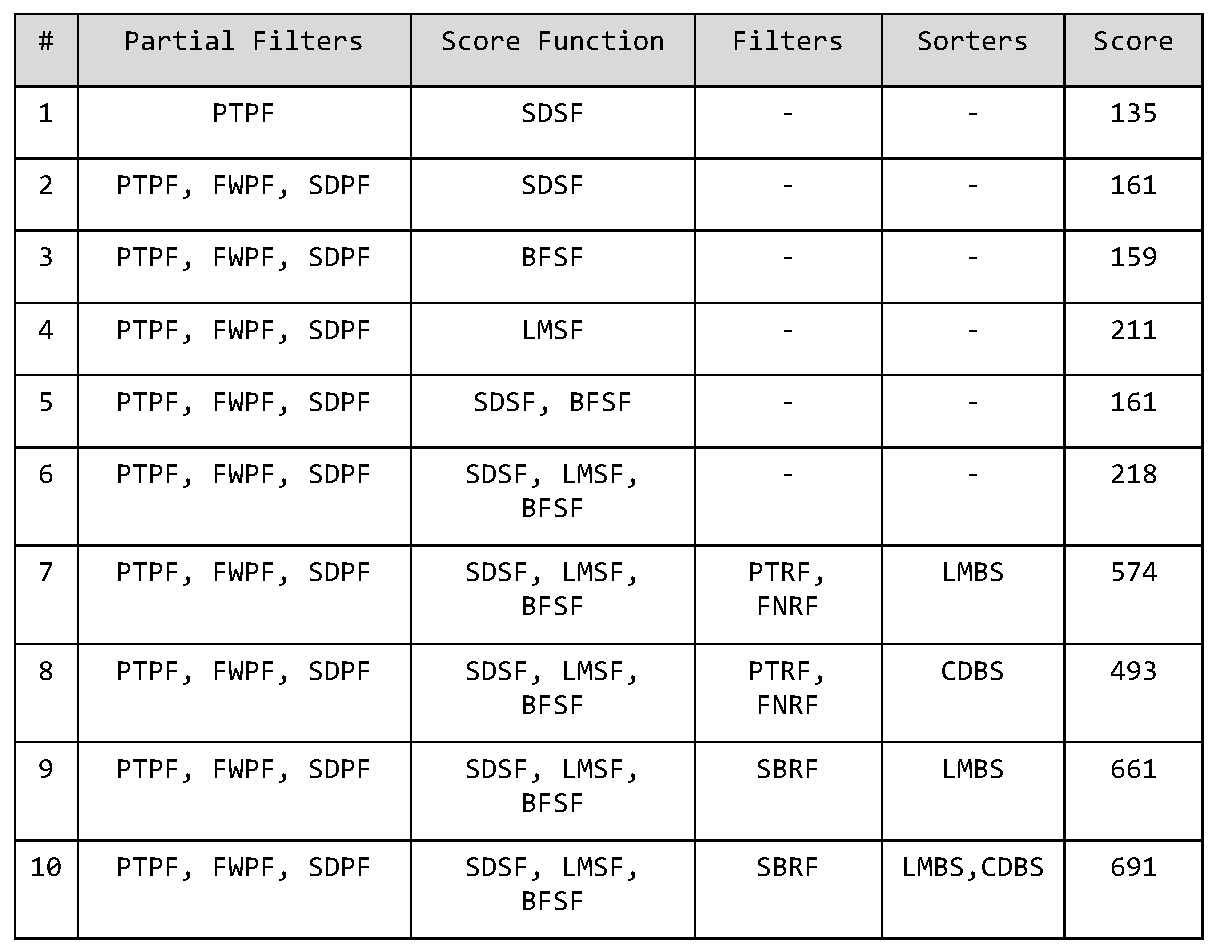
\includegraphics[scale=0.75]{g/eval-auto-results.pdf}
 \caption{Automatic evaluation results}
\end{figure}


We applied \emph{sign test} to test significance of our results. Considering $0.05$ as significance level, we found out that approaches 2 and 3 are not significantly different, as well as approaches 4 and 6. All other approaches were significantly different from each other. 

We developed a web based visualisation tool to analyse results of the automatic evaluation in greater details. This tool lists all test cases per experiment. Each item of the list is red in case of failure or green in case of success. We placed ``Details'' button in each row. Clicking this button launches a modal window which provides more details about the test case, displaying the sentence that was being translated, original paraphrasing selection, desired result and list of suggested paraphrases. This tool was implemented using JavaScript and is currently available on the project website. 

Using the visualisation tool we detected multiple problems associated with automatic paraphrases evaluation. Firstly, we noticed that our paraphraser performs significantly better in case of shorter phrases, while for longer phrases it almost always fails to find the desired paraphrase. This dependency is illustrated in Figure 4.3. However, analysing long phrases we noticed that some of them represent good paraphrasing candidates, while they do not match the original natural language English phrases. This results should be considered as success cases for paraphraser, but due to mismatch with original phrase they are classified as failure cases. If a paraphrase doesn't match the original text, it shouldn't mean a failure, it still can be a good paraphrasing option. Considering this fact our evaluation scores should be interpreted as \emph{at least} $N$ correct cases out of 2139. In order, to verify results achieved by our automatic evaluation approach we decided to carry out a user study, which will be described in the next section.

\begin{figure}
 \centering 
 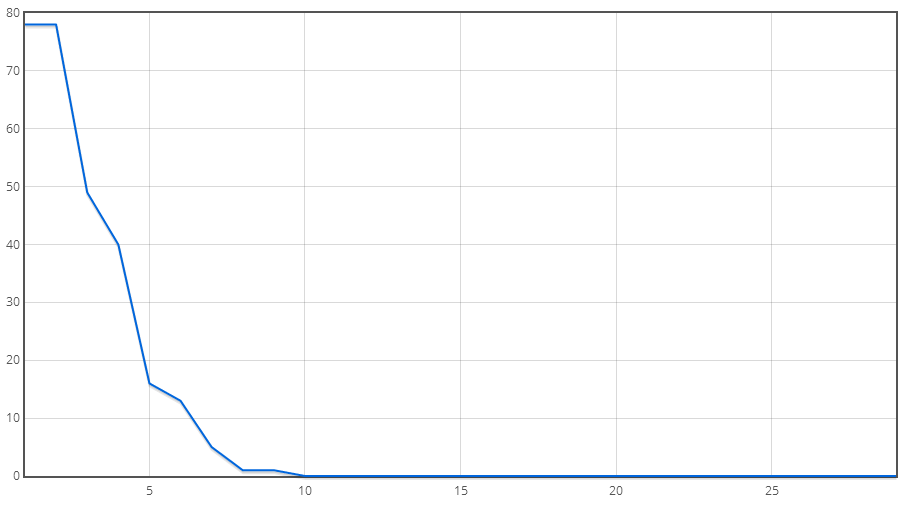
\includegraphics[scale=0.6]{g/phrase-size-chart.png}
 \caption{Relation between phrase size and paraphrasing performance}
 \caption*{X axis: number of words in phrase, Y axis: percentage of successful cases}
\end{figure}


\section{Manual evaluation}

During this project we also developed a web based interactive evaluation tool. This tool provides a user with an interface for manual evaluation of paraphrasing results. It reuses automatic evaluation test cases, displaying machine translation of the sentence. The tool also highlights an area that is considered to be corrupted as a result of alignment with original English sentences. Below the sentence we located top 5 selectable paraphrasing options that were returned by a given paraphraser version. User can pick one of these options as a better paraphrase or leave original. We also added an option for user to suggest a better paraphrase if neither options nor original text are suitable translations. Figure 4.4 illustrates the interface of our interactive evaluation tool. 

One of our goals was to make this tool easily adaptable for all paraphrasing result data we collected during automatic evaluation. To achieve this we developed a generic interface using JavaScript templating engine Handlebars.js. The data we collected during automatic evaluation stage was stored in JSON-based format and was easily rendered with our JavaScript templates.

\begin{figure}
 \centering 
 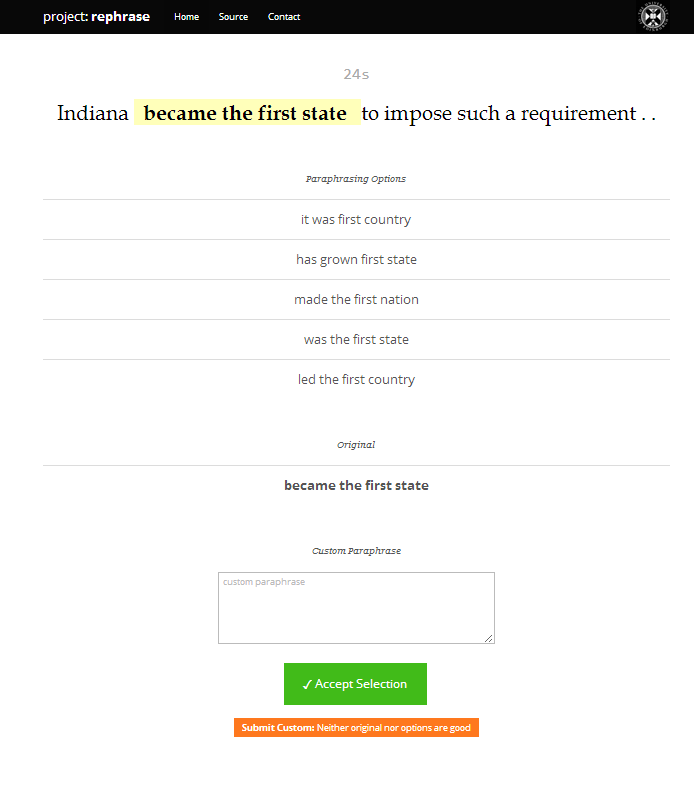
\includegraphics[scale=0.8]{g/man-eval.png}
 \caption{Manual evaluation tool}
\end{figure}

\subsection{Manual evaluation methodology}

Considering results of the automatic evaluation, we picked three out of ten tested approaches for the user study. These approaches are 1, 7 and 10. We randomly picked 50 out of our 2139 test cases, ensuring that both short and long phrases present in the final selection. We had four volunteer participants who were provided with a background information about the context of paraphrasing, they were instructed to pick a better paraphrase for selected part of sentence and to press ``Accept'', or alternatively to suggest a custom paraphrase and proceed by clicking ``Submit Custom''. 

All participants were encoded by their initials in the following way: \texttt{HG}, \texttt{OM}, \texttt{NH} and \texttt{RM}. For each of the three approaches each participant submitted his decisions for the same 50 test cases. We also considered the case when user comes across a test case that he already assessed for previous approach and his desired paraphrase selection already is in top 5 for current approaches. We automatically skipped this test cases, considering them successful. 

\begin{figure}
 \centering 
 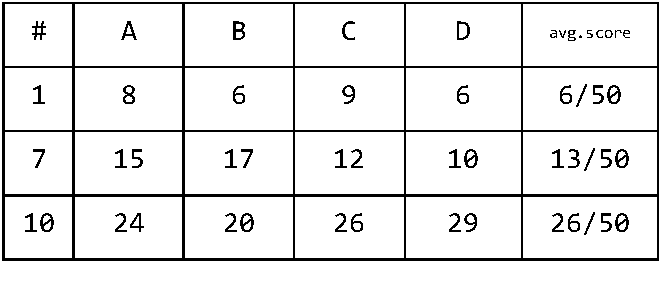
\includegraphics[scale=0.8]{g/man-eval-result.pdf}
 \caption{Manual evaluation tool}
\end{figure}

\subsection{Analysing manual evaluation results}

Final results of the user study are provided on Figure 4.5. Here the first column is approach number, four next columns contain number of successful test cases for each user. And finally last column is a unified score, which considers case successful if at least two of four annotators decided that top 5 list contains a suitable paraphrase. We can see that these results correlate with results of automatic evaluation. Indeed, applying \emph{sign test} with $0.05$ as significance level we verified that all three approaches are significantly different and most importantly that Approach 10 is significantly better than the baseline approach.